\documentclass{article}

\usepackage[utf8]{inputenc}
\usepackage{amsmath}
\usepackage{amssymb}
\usepackage{anysize}
\usepackage{color}
\usepackage{xcolor}
\usepackage{graphicx}
\usepackage{float}


\newcommand{\BigO}[1]{\ensuremath{\operatorname{O}\bigl(#1\bigr)}}

\usepackage{listings}
\lstset{
	language=C++,                	% choose the language of the code
	basicstyle=\footnotesize,       % the size of the fonts that are used for the code
	numbers= left,                 	% where to put the line-numbers
	numberstyle=\footnotesize,      % the size of the fonts that are used for the line-numbers
	stepnumber=1,                   % the step between two line-numbers. If it is 1 each line will be numbered
	numbersep=5pt,                  % how far the line-numbers are from the code
	backgroundcolor=\color{white},  % choose the background color. You must add \usepackage{color}
	showspaces=false,               % show spaces adding particular underscores
	showstringspaces=false,         % underline spaces within strings
	showtabs=false,                 % show tabs within strings adding particular underscores
	frame=single,           		% adds a frame around the code
	tabsize=2,          			% sets default tabsize to 2 spaces
	captionpos=t,          			% sets the caption-position to bottom (t=top, b=bottom)
	breaklines=true,        		% sets automatic line breaking
	breakatwhitespace=false,    	% sets if automatic breaks should only happen at whitespace
	escapeinside={\%*}{*)}          % if you want to add a comment within your code
}



\usepackage{caption}
\DeclareCaptionFont{white}{\color{white}}
\DeclareCaptionFormat{listing}{\colorbox{gray}{\parbox[c]{\textwidth}{#1#2#3}}}
\captionsetup[lstlisting]{format=listing,labelfont=white,textfont=white}

\setlength\parindent{0pt}
\setlength{\parskip}{10pt}

\marginsize{3cm}{2cm}{2cm}{2cm}

\title{Software Engineering\\
		Lab 8 Report}
\author{Emre Ozan Alkan\\
		\{emreozanalkan@gmail.com\}\\
		MSCV-5}
\date{7 December 2013}

\begin{document}
\maketitle

\section{Implementing CMatrix}
	In this lab we implemented CMatrix class to simulate a matrix and its operations like '+', '-', '*', etc.
	\subsection{CMatrix Layout}
	Here is the how CMatrix class looks like:
	\begin{lstlisting}[label=CMatrixOverview, caption=CMatrix Overview]
template<class T = int>
class CMatrix
{
private:
    vector<vector<T> > *matrix;
    int m;
    int n;
public:
	CMatrix();
	CMatrix(int size);
	CMatrix(int m, int n);
	~CMatrix();
	
	void randomize();
	void zeros();
	void identity();
	
	inline vector<vector<T> > getMatrix() const;
	inline void setMatrix(vector<vector<T> > *matrix);
	inline int getM() const;
	inline void setM(int m);
	inline int getN() const;
	inline void setN(int n);
	
	
	void fill();
	friend istream& operator>>(istream& istream, CMatrix* matrix);
	friend istream& operator>>(istream& istream, CMatrix& matrix);
	
	void display() const;
	friend ostream& operator<<(ostream& ostream, const CMatrix* matrix);
	friend ostream& operator<<(ostream& ostream, const CMatrix& matrix);
	
	void transpose();
	
	T trace() const;
	
	bool operator==(const CMatrix<T>& cmatrix) const;
	
	CMatrix<T> operator+(const CMatrix<T>& cmatrix) const;
	CMatrix<T> operator-(const CMatrix<T>& cmatrix) const;
	CMatrix<T> operator*(const CMatrix<T>& cmatrix) const;
};
	\end{lstlisting}
	

	\subsection{Constructors}
	We implemented 3 constructors. Default constructor, constructor with one parameter building identity matrix and constructor getting size of matrix and initializing it with random values.
	
	\begin{lstlisting}[label=CMatrixConstructors, caption=CMatrix Constructors]
	
    // Default Constructor: Inits empty matrix 0x0 sizes.
    CMatrix() : m(0), n(0)
    {
        matrix = new vector<vector<T> >(m, vector<T>(n, 0));
    }

    // Constructor: Getting size to build square matrix of size x size.
    // Then matrix set to identity
    CMatrix(int size) : m(size), n(size)
    {
        matrix = new vector<vector<T> >(m, vector<T>(n, 0));
        identity(); // sets matrix to identity
    }

    // Constructor: Inits the matrix with the given sizes m and n
    // Then randomly assigning values to matrix.
    CMatrix(int m, int n) : m(m), n(n)
    {
        matrix = new vector<vector<T> >(m, vector<T>(n));
        randomize(); // fills the matrix with random values
    }
    
    // Destructor: Cleaning our variables created with new keyword.
    ~CMatrix()
    {
        clog<<"CMatrix deleting..."<<endl;
        delete matrix;
        matrix = 0;
    }

	\end{lstlisting}
	
	
	\subsection{User Input and $>>$ overload}
	We created fill function to get input from user to enter coefficients of the matrix. Also this is called when $>>$ operator is used on CMatrix.
	
	\begin{lstlisting}[label=CMatrixInput, caption=CMatrix Input]
	
    // Fills the matrix with the user input
    void fill()
    {
        int i = 0, j;
        for(typename vector<vector<T> >::iterator row_it = matrix->begin(); row_it != matrix->end(); row_it++, i++)
        {
            j = 0;
            for(typename vector<T>::iterator col_it = (*row_it).begin(); col_it != (*row_it).end(); col_it++, j++)
            {
                cout<<"Please enter matrix["<<i<<"]["<<j<<"]: ";
                cin>>(*col_it);
            }
        }
    }

    // operator overloading for ">>"
    friend istream& operator>>(istream& istream, CMatrix* matrix)
    {
        matrix->fill();
        return istream;
    }

    // operator overloading for ">>"
    friend istream& operator>>(istream& istream, CMatrix& matrix)
    {
        matrix.fill();
        return istream;
    }
	\end{lstlisting}
	
	
	\subsection{Display and $<<$ overload}
	CMatrix also overloaded for $<<$ operator to display matrix itself with display function.
	
	\begin{lstlisting}[label=CMatrixDisplay, caption=CMatrix Display]
	
    // Displays the current matrix in matrix form.
    void display() const
    {
        for(typename vector<vector<T> >::iterator row_it = matrix->begin(); row_it != matrix->end(); row_it++)
        {
            for(typename vector<T>::iterator col_it = (*row_it).begin(); col_it != (*row_it).end(); col_it++)
                cout<<*col_it<<" ";

            cout<<endl;
        }
    }

    // operator overloading for "<<"
    friend ostream& operator<<(ostream& ostream, const CMatrix* matrix)
    {
        matrix->display();
        return ostream;
    }

    // operator overloading for "<<"
    friend ostream& operator<<(ostream& ostream, const CMatrix& matrix)
    {
        matrix.display();
        return ostream;
    }

	\end{lstlisting}
	
	
	\subsection{Transpose}
	We created transpose function as requested. In this function I check the current size, if it is square matrix, it getting transpose as in-place, otherwise creating another temporary matrix to hold transpose and changing it with current one.
	
		\begin{lstlisting}[label=CMatrixTranspose, caption=CMatrix Transpose]
	
    // Transposes the matrix. If square matrix,
    // just changing values across diagonal, otherwise
    // initializing new matrix with N x M, and put traspose
    // into it.
    void transpose()
    {
        // if square matrix, no need to create another matrix
        // change operations on same matrix, std::swap is used
        if(m == n)
            for(int i = 0; i < m; i++)
                for(int j = 0; j < i; j++)
                    std::swap((*matrix)[i][j], (*matrix)[j][i]);
        else
        {
            // if matrix is not square, we need to craete another matrix M x N to N x M
            vector<vector<T> > *newMatrix = new vector<vector<T> >(n, vector<T>(m, 0));

            for(int i = 0; i < m; i++)
                for(int j = 0; j < n; j++)
                    (*newMatrix)[j][i] = (*matrix)[i][j];

            delete matrix;
            matrix = newMatrix;
            newMatrix = 0;
            std::swap(m, n);
        }
    }
	\end{lstlisting}
	
	\subsection{Overloads for +, - and *}
	As all applications with matrices support addition, subtraction and multiplication, we overloaded these operators to provide similar functionality.
		\begin{lstlisting}[label=CMatrixOperations, caption=CMatrix Basic Operations]
	
    // member operator overloading for "+"
    CMatrix<T> operator+(const CMatrix<T>& cmatrix) const
    {
        if(this->m != cmatrix.m || this->n != cmatrix.n)
        {
            cerr<<"ERROR: Matrix sizes are not equal for addition..."<<endl<<"Terminating..."<<endl;
            //return 0;
            exit(EXIT_FAILURE);
        }

        CMatrix<T> tempMatrix(m, n);

        typename vector<vector<T> >::iterator row_it_current;
        typename vector<vector<T> >::iterator row_it_cmatrix;
        typename vector<vector<T> >::iterator row_it_tempmatrix;

        for(row_it_current = matrix->begin(),
            row_it_cmatrix = cmatrix.matrix->begin(),
            row_it_tempmatrix = tempMatrix.matrix->begin();

            row_it_current != matrix->end() &&
            row_it_cmatrix != cmatrix.matrix->end() &&
            row_it_tempmatrix != tempMatrix.matrix->end();

            row_it_current++,
            row_it_cmatrix++,
            row_it_tempmatrix++)
        {
            typename vector<T>::iterator col_it_current;
            typename vector<T>::iterator col_it_cmatrix;
            typename vector<T>::iterator col_it_tempmatrix;

            for(col_it_current = (*row_it_current).begin(),
                col_it_cmatrix = (*row_it_cmatrix).begin(),
                col_it_tempmatrix = (*row_it_tempmatrix).begin();

                col_it_current != (*row_it_current).end() &&
                col_it_cmatrix != (*row_it_cmatrix).end() &&
                col_it_tempmatrix != (*row_it_tempmatrix).end();

                col_it_current++,
                col_it_cmatrix++,
                col_it_tempmatrix++)
            {
                *col_it_tempmatrix = *col_it_current + *col_it_cmatrix;
            }

        }

        return tempMatrix;
    }

    // member operator overloading for "-"
    CMatrix<T> operator-(const CMatrix<T>& cmatrix) const
    {
        if(this->m != cmatrix.m || this->n != cmatrix.n)
        {
            cerr<<"ERROR: Matrix sizes are not equal for substraction..."<<endl<<"Terminating..."<<endl;
            //return 0;
            exit(EXIT_FAILURE);
        }

        CMatrix<T> tempMatrix(m, n);

        typename vector<vector<T> >::iterator row_it_current;
        typename vector<vector<T> >::iterator row_it_cmatrix;
        typename vector<vector<T> >::iterator row_it_tempmatrix;

        for(row_it_current = matrix->begin(),
            row_it_cmatrix = cmatrix.matrix->begin(),
            row_it_tempmatrix = tempMatrix.matrix->begin();

            row_it_current != matrix->end() &&
            row_it_cmatrix != cmatrix.matrix->end() &&
            row_it_tempmatrix != tempMatrix.matrix->end();

            row_it_current++,
            row_it_cmatrix++,
            row_it_tempmatrix++)
        {
            typename vector<T>::iterator col_it_current;
            typename vector<T>::iterator col_it_cmatrix;
            typename vector<T>::iterator col_it_tempmatrix;

            for(col_it_current = (*row_it_current).begin(),
                col_it_cmatrix = (*row_it_cmatrix).begin(),
                col_it_tempmatrix = (*row_it_tempmatrix).begin();

                col_it_current != (*row_it_current).end() &&
                col_it_cmatrix != (*row_it_cmatrix).end() &&
                col_it_tempmatrix != (*row_it_tempmatrix).end();

                col_it_current++,
                col_it_cmatrix++,
                col_it_tempmatrix++)
            {
                *col_it_tempmatrix = *col_it_current - *col_it_cmatrix;
            }

        }

        return tempMatrix;
    }

    // member operator overloading for "*"
    CMatrix<T> operator*(const CMatrix<T>& cmatrix) const
    {
        if(this->n != cmatrix.m)
        {
            cerr<<"ERROR: Matrix sizes are not equal for multiplication..."<<endl<<"Terminating..."<<endl;
            //return 0;
            exit(EXIT_FAILURE);
        }

        CMatrix<T> tempMatrix(this->m, cmatrix.n);
        tempMatrix.zeros();

        for(int i = 0; i < this->m; i++){
            for(int j = 0; j < cmatrix.n; j++){
                for(int k = 0; k < cmatrix.m; k++){
                    (*tempMatrix.matrix)[i][j] += (*matrix)[i][k] * (*cmatrix.matrix)[k][j];
                }
            }
        }

        return tempMatrix;
    }
	\end{lstlisting}
	
	\subsection{Overload for ==}
	We overloaded "==" operator to check if two matrices are same. If sizes are different, it returns immediately with result otherwise, it compare two matrices element wise.
	
	\begin{lstlisting}[label=CMatrixEqual, caption=CMatrix Equal Check]
	
    // member operator overloading for "=="
    bool operator==(const CMatrix<T>& cmatrix) const
    {
        if(this->m != cmatrix.m || this->n != cmatrix.n)
            return false;

        bool isEqual = true;

        typename vector<vector<T> >::iterator row_it_current;
        typename vector<vector<T> >::iterator row_it_cmatrix;

        for(row_it_current = matrix->begin(), row_it_cmatrix = cmatrix.matrix->begin(); row_it_current != matrix->end() && row_it_cmatrix != cmatrix.matrix->end(); row_it_current++, row_it_cmatrix++)
        {
//            typename vector<T>::iterator col_it_current;
//            typename vector<T>::iterator col_it_cmatrix;

//            for(col_it_current = (*row_it_current).begin(), col_it_cmatrix = (*row_it_cmatrix).begin(); col_it_current != (*row_it_current).end() && col_it_cmatrix != (*row_it_cmatrix).end(); col_it_current++, col_it_cmatrix++)
//                if(*col_it_current != *col_it_cmatrix)
//                    return false;

            isEqual = std::equal((*row_it_current).begin(), (*row_it_current).end(), (*row_it_cmatrix).begin());
            if(!isEqual)
                break;
        }

        return isEqual;
    }
	\end{lstlisting}
	
	\subsection{Trace}
	We also asked to implement CMatrix function for calculating trace of the matrix. It consecutively adding up diagonal elements of the matrix.
	\begin{lstlisting}[label=CMatrixTrace, caption=CMatrix Trace]
	
    // member operator overloading for "*"
    CMatrix<T> operator*(const CMatrix<T>& cmatrix) const
    {
        if(this->n != cmatrix.m)
        {
            cerr<<"ERROR: Matrix sizes are not equal for multiplication..."<<endl<<"Terminating..."<<endl;
            //return 0;
            exit(EXIT_FAILURE);
        }

        CMatrix<T> tempMatrix(this->m, cmatrix.n);
        tempMatrix.zeros();

        for(int i = 0; i < this->m; i++){
            for(int j = 0; j < cmatrix.n; j++){
                for(int k = 0; k < cmatrix.m; k++){
                    (*tempMatrix.matrix)[i][j] += (*matrix)[i][k] * (*cmatrix.matrix)[k][j];
                }
            }
        }

        return tempMatrix;
    }
	\end{lstlisting}
	
	\subsection{Helper Functions}
	Here is the some other function implemented in CMatrix as helper functions.
	\begin{lstlisting}[label=CMatrixHelper, caption=CMatrix Helper Functions]
	
    // Randomly initialize the matrix that inside the class between 0 and 5
    void randomize()
    {
        for(typename vector<vector<T> >::iterator row_it = matrix->begin(); row_it != matrix->end(); row_it++)
            for(typename vector<T>::iterator col_it = (*row_it).begin(); col_it != (*row_it).end(); col_it++)
                *col_it = T(rand() % 5);
    }
    
    // Fill the matrix with zeros.
    void zeros()
    {
        for(typename vector<vector<T> >::iterator row_it = matrix->begin(); row_it != matrix->end(); row_it++)
            for(typename vector<T>::iterator col_it = (*row_it).begin(); col_it != (*row_it).end(); col_it++)
                *col_it = T(0);
    }
    
    // Converts current matrix to identity matrix
    void identity()
    {
        if(m != n)
            clog<<"identity() on non-square matrix"<<endl;

        zeros();

        // We need to know minimum of the size to traverse on diagonal
        int diogonalCount = std::min(m, n);

        typename vector<vector<T> >::iterator it_row;
        typename vector<T>::iterator it_col;

        // We going to iterate diogonalCount times our iterators
        for(int i = 0; i < diogonalCount; i++)
        {
            it_row = matrix->begin();
            for(int j = 0; j < i; j++) // iterate through current diagonal element for row
                ++it_row;

            it_col = (*it_row).begin();
            for(int k = 0; k < i; k++) // iterate through current diagonal element for column
                ++it_col;

            *it_col = T(1); // set the (i, i). diogonal element to 1
        }
    }
    
    
	\end{lstlisting}
	
	
	\subsection{Result}
	Here is the example main and the output of the program.
	\begin{lstlisting}[label=CMatrixMain, caption=Example Main]
	
int main(int argc, char **argv, char **env)
{
    atexit(allLabsFinished);
    path = argv[0];

    srand(time(NULL));

    CMatrix<> matrix1(2);
    CMatrix<> matrix2(2, 2);

    cout<<"Matrix 1:"<<endl;
    cout<<matrix1;
    cout<<"Matrix 2:"<<endl;
    matrix2.display();

    cout<<"Please fill the Matrix 1:"<<endl;
    matrix1.fill();
    cout<<"Please fill the Matrix 2:"<<endl;
    cin>>matrix2;

    cout<<"Matrix 1:"<<endl;
    matrix1.display();
    cout<<"Matrix 2:"<<endl;
    cout<<matrix2;

    cout<<"Trasposing Matrix 1:"<<endl;
    matrix1.transpose();
    cout<<"Transposing Matrix 2:"<<endl;
    matrix2.transpose();

    cout<<"Matrix 1:"<<endl;
    cout<<matrix1;
    cout<<"Matrix 2:"<<endl;
    matrix2.display();

    auto matrixAdd = matrix1 + matrix2;
    auto matrixSub = matrix1 - matrix2;
    auto matrixMul = matrix1 * matrix2;
    auto matrixEql = (matrix1 == matrix2);
    auto matrix1Trace = matrix1.trace();
    auto matrix2Trace = matrix2.trace();

    cout<<"Result of Matrix 1 + Matrix 2:"<<endl;
    matrixAdd.display();
    cout<<"Result of Matrix 1 - Matrix 2:"<<endl;
    cout<<matrixSub;
    cout<<"Result of Matrix 1 * Matrix 2:"<<endl;
    matrixMul.display();
    cout<<"Result of Matrix 1 == Matrix2"<<endl;
    if(matrixEql)
        cout<<"Matrices are equal"<<endl;
    else
        cout<<"Matrices are NOT equal"<<endl;
    cout<<"Trace of Matrix 1:"<<endl;
    cout<<matrix1Trace<<endl;
    cout<<"Trace of Matrix 2:"<<endl;
    cout<<matrix2Trace<<endl;

    return 0;
}
	\end{lstlisting}
	
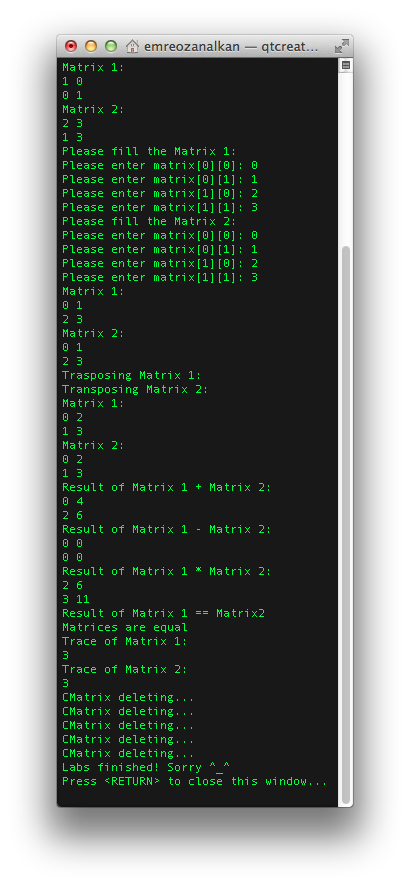
\includegraphics[scale=0.8]{Lab8Result.png}


\end{document}







































